\documentclass[fleqn]{article}

%% Language and font encodings
\renewcommand{\familydefault}{\sfdefault} % use sans serif per default
\usepackage{helvet} % use helvetica per default

\usepackage[english]{babel}
\usepackage[utf8]{inputenc}
\usepackage[T1]{fontenc}

%% Sets page size and margins
\usepackage[a4paper,top=1.5cm,bottom=1.5cm,left=2cm,right=2cm,marginparwidth=1.75cm]{geometry}

%% Useful packages
\usepackage{amsmath,amssymb} % for advanced math formulas
\setlength{\mathindent}{0pt}
\usepackage{hyperref}
\usepackage{graphicx}

\title{Status report - Deep learning with Siamese networks for instance search or identification}
\author{Matthias Kohl}

\begin{document}
\maketitle

This report serves as a status report for the internship on
Siamese networks for instance search (image retrieval),
supervised by Georges Quénot and Jean-Pierre Chevallet,
in collaboration with Maxime Portaz.

This report should not be seen as a scientific report.
Instead, it is a simple overview of the main ideas and
results of the internship so far and will be updated on the fly.

\section{Introduction}
We consider the problem of instance search for images.
The goal is as follows:
given a reference dataset of images and a query image,
retrieve the image from the reference dataset that
best suits the query image.

This problem is related to image classification:
if we consider each instance of an object as a class,
we can classify the query image and return any image
from that class in the reference dataset.

The difference with image classification is that
there is almost no variability within the classes,
as they are in fact a single object.
So the objective is to focus more on differentiating between objects,
rather than predicting the type of object.
Thus for a given query image, we try to tell how much it resembles each
image of the reference dataset.

\section{State of the art}
Previously, most systems were based on a bag-of-words approach
in order to match images~\cite{philbin_object_2007}.
Combined with better techniques of matching the bag-of-words descriptors,
this approach was previously the state-of-the-art~\cite{mikulik_learning_2013}.

Recently, the state-of-the-art has drastically improved due to the
addition of learned features, based on convolutional neural networks
(CNNs).
This new approach greatly improved
mean average precision scores~\cite{gordo_deep_2016} of the system
on the same datasets.

The general trend is to move from an approach based on a combination of
engineered features (bag-of-words combined with
support vector machines or SVMs) to a more end-to-end learning of
the matching of two images.

For this, the Siamese architecture is used, where the convolutional
features of two or more CNNs with shared weights are combined and a
multi-way loss is optimized, which discriminates between the features
of two or more images.
This concept was first introduced by
Chopra et al~\cite{chopra_learning_2005} to learn a dissimilarity metric
between two images.

For a learning-to-rank setting, this idea was extended to a triplet loss
by Weinberger et al~\cite{weinberger_distance_2006}.
This loss is better suited when learning to rank, rather than instance
search, but it also allows for a more stable convergence, which is
beneficial in both cases.

Using this triplet loss has achieved state-of-the-art results in both
face recognition~\cite{schroff_facenet:_2015} and
image retrieval~\cite{gordo_deep_2016}. This is mostly due to the usage
of far deeper CNNs, moving from architectures such as
AlexNet~\cite{krizhevsky_imagenet_2012} to VGG~\cite{simonyan_very_2014}
and finally Inception~\cite{szegedy_inception-v4_2016} and
ResNet~\cite{he_deep_2015}.

The higher depth of networks like ResNet and Inception as compared to
AlexNet allows for higher regularization and thus less over-fitting
to a specific dataset for these architectures. Batch normalization
increases this effect even more. This is a desirable trait for image
retrieval, as the variability within each instance is too small to
learn classification directly. So the better we can generalize
features learned from a bigger dataset to the reference dataset,
the better performance we can expect.

\section{Evaluation}\label{sec:eval}
We are using the following datasets in our experiments:
\begin{enumerate}
    \item CLICIDE: dataset of photographs taken in an art museum,
    consisting exclusively of paintings. The dataset is characteristic
    because the different images for each instance consist of one
    global view of the instance and multiple sub-parts.

    Number of reference images: 3245 (the full dataset contains
    3452 images with 207 images of walls and no meaningful instance)
    Number of test images: 165 (the full dataset contains 177
    test images, out of which 165 share their instance with
    at least one image of the reference set)
    Number of instances: 464
    \item GaRoFou\_I: dataset of photographs of an art museum,
    consisting of display cabinets, which contain sculptures,
    rocks and various types of objects.

    Number of reference images: 1068
    Number of test images: 184 (all are used for evaluation)
    Number of instances: 311
    % \item GaRoFou_V: dataset of frames from a video taken by visitors
    % of the same museum as above.

    % Number of reference images: 2779
    % Number of test images: 2132
    % Number of instances: 215
    % \item Oxford5k: dataset of photographs of buildings taken in
    % the city of Oxford, UK.

    % Number of reference images: 5000 TODO
    % Number of test images: 55 TODO
    % Number of instances: 17 TODO
\end{enumerate}

\subsection{Evaluation metrics}
\subsubsection{Metrics definitions}
\paragraph{$Precision@k$}
For a test image and $m$ reference images and a ranking of the
reference images $I_1, \dots, I_m$, we define the number of relevant
images at $k$ with $k \leq m$:
$N^{rel}_k$ is the number of images in the sub-ranking
$I_1, \dots, I_k$ from the same instance than the test image.

We then define Precision at $k$ as:

\begin{equation}
Precision@k = \frac{N^{rel}_k}{k}
\end{equation}

\paragraph{MAP}
As above, for a test image, $m$ reference images and a ranking
of the reference images, we define the average precision:

\begin{equation}
AP = \frac{1}{N^{rel}_m} \sum_{k=1}^m Precision@k
\end{equation}

The MAP score is defined as the mean of the AP score over all test images.

\subsubsection{Used metrics}
As of now, we use the mean $Precision@1$ to evaluate the system.
It is the mean of the $Precision@1$ for all test images.
This is what we are most interested in: in the context of a
search system for retrieving art in a museum, we are only
interested in one result, as the user should not make a choice
out of several results.

To be comparable with other papers in the field, we will implement
the MAP score as well later on.

\section{Methodology}
The following approaches have been tested:

\subsection{Features of a pre-trained CNN}\label{sec:cnnplain}
We use the features obtained from a CNN that was pre-trained on ImageNet.
The feature dimension of the last layer is thus
fixed at 1000, the number of classes in ImageNet.

We also use the convolutional features obtained from such a CNN.
Their dimensions are specified in{} the specifics section.
\subsubsection{Motivation}
This is to set a baseline for other approaches and to reproduce results
from a previous paper (TODO cite CORIA paper).
\subsubsection{Specifics}
All images are resized to $224 \times 224$, using a bilinear
re-sampling filter. This is to fit the default input dimensions of
a CNN used in ImageNet.

The following CNNs were tested:
\begin{enumerate}
    \item AlexNet (convolutional feature dimension $6 \times 6 \times 256 = 9216$)
    \item ResNet-152 (convolutional feature dimension $7 \times 7 \times 2048 =100352$)
\end{enumerate}

\subsection{Features of a fine-tuned CNN}\label{sec:finetune}
We use the features obtained from a CNN, pre-trained on ImageNet,
then fine-tuned as a classification net on the reference dataset.

The feature dimensions are much smaller and correspond to the number
of instances of the dataset, described in Section~\ref{sec:eval}.

Similarly to the approach in Section~\ref{sec:cnnplain},
we also use the convolutional features obtained from a fine-tuned model,
having the same dimensions than described there.
\subsubsection{Motivation}
The idea is to fine-tune the high-level convolutional filters
to our dataset such that they can capture the shapes of that dataset better.
\subsubsection{Specifics}\label{sec:finetunespecs}
All images are resized to $224 \times 224$, using a bilinear
re-sampling filter.

For fine-tuning the CNN on classification, we use the following settings:
\begin{enumerate}
    \item Data augmentation: all images are shifted (in range $[-20\%, 20\%]$ in both directions), rotated (in range $[-45, 45]$ degrees), rescaled (with factor in range $[0.8, 1.2]$) and horizontally flipped at random.
    All parameters are chosen from a uniform distribution.

    The motivation behind the extensive data augmentation is that
    the training set is very small, so without data augmentation,
    large CNNs like AlexNet would over-fit the dataset.
    \item Number of epochs: $50$
    \item Learning rate: $0.01$ (annealed by a factor of $0.1$ after 30 epochs)
    \item Momentum: $0.9$
    \item Weight decay: $0.0005$
\end{enumerate}

Note that the hyper-parameters were chosen manually without optimization
since they appeared to work well on the CLICIDE dataset. This means they
might be far from optimal on both datasets, and especially GaRoFou.

The following CNNs were tested:
\begin{enumerate}
    \item AlexNet (only last convolutional layer is fine-tuned)
    \item ResNet-152 (last 3 blocks are fine-tuned)
\end{enumerate}

\subsection{Features of a fine-tuned Siamese CNN using cosine similarity loss}
The general principle follows the architecture of
Gordo et al~\cite{gordo_deep_2016}, omitting the region pooling:
We use the convolutional features of a pre-trained CNN.
These features are $L2$-normalized, then a shifting layer and
fully connected layer are introduced to reduce the
feature dimension and the features are
$L2$-normalized again. This is similar to the architecture of
Schroff et al~\cite{schroff_facenet:_2015}, too.

Most importantly, we use a Siamese architecture along with a cosine
similarity loss. The loss is defined as follows for two images and
their feature vectors $x_1$ and $x_2$:

\begin{equation}
\mathcal{L} =
\begin{cases}
1 - cos(x_1, x_2) & \text{if the images are from the same instance}\\
\max(0, cos(x_1, x_2) - margin) & \text{if the images are from different instances}
\end{cases}
\end{equation}

$cos(x_1, x_2) = \frac{x_1 x_2}{\|x_1\|_2 \|x_2\|_2}$. For normalized
vectors, we have $cos(x_1, x_2) = x_1 x_2$, so the cosine similarity is
simply the dot product here.

\subsubsection{Motivation}
On small datasets, Siamese architectures should be able to obtain better
results than classification architectures as they are fine-tuned to
discriminate between two inputs, rather than simply output the class or
instance of an input.
Because of the missing variability for each instance, a classification
architecture will over-fit the dataset more than a Siamese architecture.

As described above, we omit the region pooling layer. There are two
reasons behind this: First, we only use images of the same size
as inputs, so we do not need to harmonize between different images.
Second, the images in our datasets are cleaner than images in the
datasets used by Gordo et al (Oxford5k, Paris6k, \dots), in the sense
that the objects are usually well centered in the images and fill out
most of the image. In other datasets, the objects searched for
only form a small part of the image. In this case, the rest of the image
is noise, making the network more difficult or impossible to train.

\subsubsection{Specifics}
All images are resized to $224 \times 224$, using a bilinear
re-sampling filter. The margin in the loss is set to 0.

For fine-tuning the Siamese CNN, we use the following settings:
\begin{enumerate}
    \item Margin used in loss: $margin:=0$
    \item Data augmentation: None/same as in fine-tuning
    (Section~\ref{sec:finetunespecs})
    \item Batch size: 64/256
    \item Number of epochs: $50$
    \item Learning rate: $0.001$
    \item Momentum: $0.9$
    \item Annealing: None
\end{enumerate}

The following choices of the pairs of images for training were tested:
\begin{enumerate}
    \item Choose all positive pairs and randomly choose negative pairs
    such that $90\%$ of the training set consists of negative pairs
    \item Choose all positive pairs and for each image, choose the
    'hardest' $x$ negative pairs: the pairs giving the highest loss.
    This choice of the hardest pairs is repeated before each epoch
    during training.
\end{enumerate}

The following CNNs were tested:
\begin{enumerate}
    \item AlexNet (only last convolutional layer is fine-tuned)
    \item ResNet-152 (last 3 blocks are fine-tuned)
\end{enumerate}

\subsection{Features of a fine-tuned Siamese CNN using a triplet loss}
This resembles the architecture of Gordo et al~\cite{gordo_deep_2016}
the most: only region pooling of the convolutional features is omitted.

The loss is defined for an anchor image, a reference positive image and
a reference negative image and their feature vectors $x_a$, $x_p$, $x_n$
respectively:

\begin{equation}
\mathcal{L} = \frac{1}{2}
\max(0, \| x_a - x_p \|_2^2 - \| x_a - x_n \|_2^2 + margin)
\end{equation}

For normalized feature vectors $x_1$, $x_2$, the distance $\| x_1 - x_2\|$
between the vectors is closely related to the cosine similarity:
$\| x_1 - x_2 \|_2^2 = 2-2x_1x_2 = 2-2cos(x_1,x_2)$.
So the loss could be written as
$\max(0, x_ax_n - x_ax_p + margin^{\star})$ with
$margin^{\star} = \frac{1}{2} margin$. Both versions of the loss
are implemented, but we chose the margin $margin^{\star}$ as basis
since in our case, feature vectors are always normalized.

\subsubsection{Motivation}
The motivation behind using the triplet loss is laid out in the paper
by Weinberger et al~\cite{weinberger_distance_2006}, who first introduced
this loss, as well as the paper by Schroff et al~\cite{schroff_facenet:_2015}.
Essentially, this loss is more robust w.r.t. noise in the data, as
we cannot always perfectly project all couples of images of the same
instance onto the same point in space, when we have noisy data.

\subsubsection{Specifics}
All images are resized to $224 \times 224$, using a bilinear
re-sampling filter. The margin in the loss is set to 0.

For fine-tuning the Siamese CNN, we use the following settings:
\begin{enumerate}
    \item Margin used in loss: $margin^{\star}:=0.2$
    \item Data augmentation: None/same as fine-tuning
    (Section~\ref{sec:finetunespecs})
    \item Batch size: 64/256
    \item Number of epochs: $50$
    \item Learning rate: $0.001$
    \item Momentum: $0.9$
    \item Annealing: None
\end{enumerate}

The following choices of the triplets of images for training were tested:
\begin{enumerate}
    \item Choose all positive pairs and randomly choose a negative pair
    for each positive pair to form a triplet.
    \item Choose all positive pairs and for each image, choose the
    'hardest' negative pair to form a triplet.
    \item Choose all positive pairs and for each image, choose 'semi-hard'
    negatives early on in training, then choose only the 'hardest'
    negatives. This is motivated by Schroff et al~\cite{schroff_facenet:_2015}.
    \item Choose the easiest $n_p$ positives along with the
    hardest $n_n$ negatives. Then compute the loss for all $n_p\times n_n$
    triplets. Choose the $n_t$ triplets with the highest loss.
    Repeat this procedure until a large enough number of hard triplets
    are found. Perform this before each epoch during training.
    This is motivated by the strategy of Gordo et al~\cite{gordo_deep_2016}.
\end{enumerate}

The following CNNs were tested:
\begin{enumerate}
    \item AlexNet (only last convolutional layer is fine-tuned)
    \item ResNet-152 (last 3 blocks are fine-tuned)
\end{enumerate}

\section{Results}
Table~\ref{tab:results} shows current results for each approach.
The following special values can appear in the table:
\begin{itemize}
    \item N/A: configuration was not tested
    \item CH: loss gets smaller, but converges at a high value.
    usually in this case, testing performance stagnates or goes slightly down.
    We tried different batch sizes, but none give a better result.
    This usually indicates that we always converge to a local minimum
    or the model collapses (setting all embeddings to 0 for example)
    \item CBT: loss converges towards 0, but testing performance does
    not improve. this shows the model performs bad somehow
\end{itemize}

All new results are added there as soon as available.

\begin{table}
\begin{tabular}{|c|c|c||c|c|}
\hline
Approach & \multicolumn{4}{|c|}{Dataset}\\
\hline
& \multicolumn{2}{|c||}{CLICIDE} & \multicolumn{2}{|c|}{GaRoFou\_I}\\
\hline
& AlexNet & ResNet-152 & AlexNet & ResNet-152\\
\hline
% TODO: verify results for GaRoFou now
Full classif. features of pre-trained net
& 57.58 & 64.24 & 76.63 & 75.54 \\
\hline
Conv. features of pre-trained net
& 72.73 & 75.76 & 85.33 & 84.78 \\
\hline
Full classif. features of classif.-fine-tuned net
& N/A & 77.58 & 86.96 & 92.93 \\
\hline
Conv. features of classif.-fine-tuned net
& N/A & 89.70 & 89.13 & 96.20 \\
\hline
Classif fine-tuned semantic sub-regions
& N/A & 94.55 & N/A & N/A \\
\hline
Cosine loss (random pairs) with pre-trained net
& N/A & N/A & N/A & N/A \\
\hline
Cosine loss (hardest pairs) with pre-trained net
& N/A & N/A & N/A & N/A \\
\hline
Triplet loss (all pos, random neg) with pre-trained net
& N/A & CBT & N/A & N/A \\
\hline
Triplet loss (all pos, semi-hard neg) with pre-trained net
& N/A & 86.06 & N/A & N/A \\
\hline
Triplet loss (easy pos, hard neg) with pre-trained net
& N/A & CBT & N/A & N/A \\
\hline
Triplet loss (semi-hard), semantic sub-regions
& N/A & 92.73 & N/A & N/A \\
\hline
\end{tabular}
\caption{Results in percentage points of mean $Precision@1$ of various approaches on different datasets and underlying networks\label{tab:results}}
\end{table}

\section{Current work}
\begin{itemize}
    \item Obtain results for various approaches and datasets. See how well
    the different approaches generalize.
\end{itemize}

\section{Future work}
\begin{itemize}
    \item Propose new approach: This could be based on ideas from the
    following papers:
    \begin{enumerate}
        \item Conditional similarity networks,
        Veit et al~\cite{veit_conditional_2016}
        \item Learning to remember rare events (few-shot classification),
        Kaiser et al~\cite{kaiser_learning_2017}
    \end{enumerate}
    \item Possibly add more visualizations to see whether the filters
    capture the images as expected: There are several approaches.
    \begin{enumerate}
        \item Show the gradient for single filter activation:
        class saliency extraction, not implemented yet
        \item optimize response of filter +
        regularized image by gradient descent (keeping weights fixed):
        for this and previous approach, see paper by
        Simonyan et al 'Deep Inside Convolutional Networks..':
        not implemented yet
    \end{enumerate}

    \item Possibly create new dataset
    (based on images of museum art pieces)

    Motivation: CLICIDE dataset is particularly suited for ORB.
    GaRoFou dataset is very small, so the risk of over-fitting
    to that particular type of dataset is high.

    A better dataset would be one with more images
    (and proportionally more instances) and a better harmonization of
    query vs reference images: reference images should be clean and from
    all angles of the object, query images should not be clean, blurred,
    only small parts of the image contains object to find \dots
\end{itemize}

\section{Past work}
\begin{itemize}
    \item Tested Gordo's system directly on our dataset
    \item Investigated discrepancies between our results and CORIA results.
    In part, this seems to be due to how the dataset is read (correct
    orientation or not), how the normalization is performed and how the
    results are calculated precisely (this is not available atm)

    Indeed, because the datasets are small, simply choosing a different
    normalization can have a big impact on results
    (image-wise normalization vs
    dataset-wise normalization and in case of dataset-wise, there are
    different possible ways to do that: pixel-wise \dots)

    \item Created simple visualizations to see which results are failing,
    feature maps of filters, plots for loss evolution, heat map and
    classification map for fully convolutional network

    \item Identified issue in CLICIDE dataset: it seems like the images
    that are not being retrieved have a different scale than all reference
    images

    \item Identified discrepancies between our problem and Oxford5k/Paris6k:
    Oxford and Paris datasets contain many images unrelated to the actual
    objects that are being queried. They are more general image retrieval
    datasets, where we want to find similar images out of (many) irrelevant
    images. Our datasets (CLICIDE and GaRoFou) are identification datasets,
    where we want to identify the correct object out of many possible ones.

    Hence, the proposed approach cannot work properly on Oxford/Paris, unless
    we assume that we already know the images that actually represent the
    same object: this is what Gordo achieves in cleaning his large dataset,
    plus the large dataset is very similar to Oxford/Paris. This is
    impractical though as for a different dataset, this means having a
    large, clean dataset with similar images available

    \item Proposed and implemented the following approach:
    \begin{itemize}
        \item Transform fine-tuned classification net into fully
        convolutional network (FCN) as suggested by
        Long et al~\cite{long_fully_2015}. Figure~\ref{fig:fcn} shows
        how this is achieved. Evaluating the fully convolutional network
        on an arbitrarily-sized image is the same thing as evaluating it
        by sliding it over the input with the stride of the net (this is
        32 for both AlexNet and ResNet, but for AlexNet, it would start
        slightly outside the frame of the input image) and the ideal
        input region of the net (223x223 for AlexNet, 224x224 for ResNet)
        \item Only consider locations of the highest activations
        in the classification map. This should correspond to the
        approximate region of interest
        \item for each region, perform the same transformation than
        in Gordo's paper (Shift + FC layer, normalize),
        then sum-accumulate over the regions and normalize again
    \end{itemize}
    \item Proposed and implemented another approach based on classification:
    \begin{itemize}
        \item Transform fine-tuned classification net into fully
        convolutional network (FCN)
        \item Simply enforce classification for all sub-regions of an image.
        Do this with a scaled version of the image, too. The classifier
        should be particularly robust to scale changes. This may require
        fine-tuning far more layers than what we're currently doing to be
        efficient.
    \end{itemize}
\end{itemize}

\begin{figure}
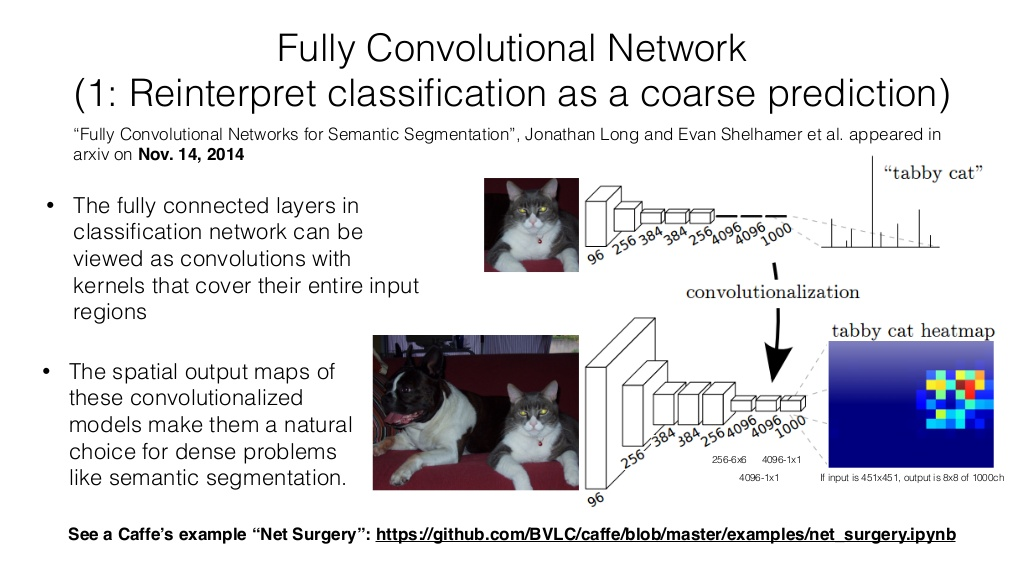
\includegraphics[width=\textwidth]{fcn_slide.jpg}
\caption[caption]{Convolutionalization of fully connected layers
\\\hspace{\textwidth}source:
\url{https://www.slideshare.net/mitmul/
a-brief-introduction-to-recent-segmentation-methods}\label{fig:fcn}}
\end{figure}


\bibliographystyle{ieeetr}
\bibliography{siamese}

\newpage
\appendix
\section{Implementation details and specifics}
\subsection{General issues}
large images/large batch sizes/large nets means we require lots of memory
this means we implement so-called micro-batches for gradient descent:
each mini-batch is decomposed into several micro-batches.
perform a forward pass over the micro-batches while accumulating the loss.
then, perform a backward pass, which is representative of the mini-batch,
but we require only as much memory as for one micro-batch


be careful when training with micro-batches. this is required here because
of memory issues. however, there can be some issues:
    - averaging the loss needs to be done correctly if an average loss
    is wanted. each micro-batch loss needs to be scaled by a factor n/m
    where n is the size of the micro-batch and m the mini-batch size
    - The BatchNorm layer does not work as expected with very small
    micro-batches, since it computes a running mean and variance during
    training. this cannot work if only 1 or 2 images are given per batch.
    In PyTorch, this kind of layer needs to be set in eval mode instead
    if small micro-batches are used. However, this means the parameters
    (global mean/var approx) need to be calculated up-front, for example
    during classification where bigger batch sizes can be used

\subsection{Library issues}
PIL ignores EXIF 'Orientation' tag, while almost all image viewers don't.
This means PIL reads camera images where the camera was rotated as rotated
images. OpenCV seems to handle this case correctly, instead.

\subsection{PyTorch specific issues}
TODO

\end{document}
